\chapter{Literature Review}\label{chap:litreview}

\section{Deep Learning and MDP Homomorphisms}
As discussed previously In Chapter \ref{chap:background} the idea of learning a Group Structured MDP homomorphism is a powerfull tool to make the learning problem posed by an MDP simpler. In this section I will discuss multiple parpers that attempt to learn Group Structured MDP Homomorphisms.
\subsection{MDP Homomorphic Networks}
\cite{vanderpol2020mdp} introduces the idea of performing policy based learning that respects the symmetry of the environment, by constraining the possible policies that can be represented by a neural network.

This is achieved by using an equivariant network on discrete action spaces. When the input to the network is transformed by a group structured operation, the output policy is also transformed by this operation, due to the equivariance property, and as such the network finds a more efficient method of learning the policy as the MDP problem it is solving is simpler, as it exploits the Group Structured MDP Homomorphism.

The equivariance in the deep network uses many of the same ideas as that of the G-CNNs\cite{cohen2016group}. In that the only requirement for a network to be equivaraint to a discrete group action's is that the individual layers of the network are equivariant to the group's actions. Despite the similarity, thier method of achieving the equivariance is quite different. The Authors propose the "symmetrizer layer". In contrast to the group convolution formulation, the symmetrizer layer achives equivaraince by finding weight matricies that are solutions to,
\begin{equation}
	\label{eqn:symmetrizer}
	\mat{W} =S(\mat{W}) = \frac{1}{|G|}\sum_{g\in G}{\pi_g^{\mathcal{X}'}}^{-1}\mat{W}\pi_g^{\mathcal{X}}
\end{equation}
Where if $f(\vec{x}) = \mat{W}\vec{x}$, $f: \mathcal{X} \rightarrow {\mathcal{X}'}$ and $\pi_g^{\mathcal{X}}$ is the representation of $g$ in $\mathcal{X}$, then $\pi_g^{\mathcal{X}'}$ is the representation of $g$ in $\mathcal{X}'$. In order to find such linear systems of equations in a general manner for a group $G$, the authors sample many matricies randomly from the space of all possible matricies of that size $\mathcal{W}_{total}$.Then apply the symmetrizer operation, $S$, to all of the sampled matricies.


From this point, because the symmetrizer operation is linear there exists a set of solutions to that linear equation,$\mathcal{W}$, and to form solutions to it, they vectorise and stack the found matricies, This forms a new matrix, which the singular value decomposition's basis vectors are orthogonal vectors of the equivariant subspace! These vectors $\{\mat{V}_i\}$ are all solutions to the above equation\ref{eqn:symmetrizer}. As such any linear combination of them is also a solution. Using the first $r$ vectors of the SVD, where $r= \text{rank}(\mathcal{W})$. An equivariant layer can by formed by,

\begin{equation}
	\mat{W} = \sum_{i=1}^{r}{\alpha_i\mat{V}_i}
\end{equation}

These layers have interesting properties in that the size of the subspace defines how many parameters when using this framework, there is no current closed form solution to the question of how many parameters each layer will have.

This scheme of producing equivariant layers, has some notable upsides, in that you only need to know how to trasform the input and output of the layer, $\mat{W} \rightarrow \mat{W}\pi_g^\mathcal{X}$ and $\mat{W} \rightarrow {\pi_g^{\mathcal{X}'}}^{-1} \mat{W}$ respectively. However, the scheme does require, expensive SVD calculations, in addition to the sampling of many matricies, which is expensive, but this only need be done once at the start of training per layer. However, there is no closed form solution to how many parameters the matricies will have, and as such the number of parameters in the network is not known until the SVD is performed.

The larger problems with this approach are that the homomorphisms must be exact, and known apriori. This limits the possible scenarios in which this approach can be used, as it is not always possible to know the exact symmetry. In addtion, to this in many cases generalising to continuous actions spaces is not possible with the current methodology.


\subsection{Group Equivariant Deep Reinforcement Leanrning}
In much the same vein as that of \cite{vanderpol2020mdp}, \cite{mondal2020group} proposes a method of exploiting equivariant networks for Deep RL, in comparison to \cite{vanderpol2020mdp}, they propose using G-CNNs\cite{cohen2016group} to achieve equivariance, rather than the symmetrizer layer. In contrast to leaning a policy they have a newtwork structure such that the states are mapped to an equivariant Latent space of dimension 256, This results in a network architure that can be thought of as an equivariant embedding function, $f(s)$, and a Q-Value function, $Q(s_{eqv}, a)$, acting on this space.
\begin{align}
	f: & \mathcal{S} \rightarrow \mathcal{S}_{eqv}      \\
	Q: & \mathcal{S}_{eqv} \rightarrow \mathbb{R}^{|A|}
\end{align}

One of the key downsides of this is it doesn't exploit the homomorphism of the MDP, that exists also in the action space. Despite this \cite{mondal2020group} still demonstrate an improvement in sample efficiency over a baselines of DDQN~\cite{van2016deep} and DQN~\cite{mnih2013playing} in snake. However, they onlt see a minor improvement in sample efficiency in Pacman, which also posseses the same $C_4$ group symmetry.

\subsection{$\mathrm{SO}(2)$ Equivariant Reinforcement Learning}

In much the same way as the above methods,~\cite{wang2022so2} also exploit exploit the equivariance property, in the context of robotic control in the PyBullet suite\cite{coumans2021}. They use steerable G-CNNs\cite{weiler2019general}, which provide $\text{SE}(2)$ equivariance, in robotic control environments. In contrast to previous papers where finite groups were exploited, the continuous Lie group $\text{SO}2$ constrains the degrees of freedom of the problem much more than the finite groups. Utilising this they are able to achieve impressive improvements in sample efficiency and robustness over conventional DQN and SAC mtehods.

In their first experiments of Drawer-Opening, Block Pulling, and Object Picking, the equivariant networks outperform all other DQN methods, and when applied to the SAC forumlation, In Objedct picking and Drawer Opening, they are the only methods that are able to solve the task.

Further they perform tests on more difficult robotic control tasks where demonstrations are provided, this enables the the agents to tackle more complex tasks such as block stacking and house building, in which they again are the only agents that are able to solve the tasks.


\section{Learning Models}
In the context of exploiting symmetries in RL, there is also the opportunity, to build world models which are learned from experience. Two possible approaches are, learning a world model using an network that is equivariant to the group actions, in this case, the world model has the same state action space as the origional MDP, however, the equivariance inductive bias may improve the sample efficiency of learning the world model, and introduces better generalisation, for the agent. In some ways this is the model based extension of the equivariant model free methods discussed above.

An alternative approach is to learn a world model that is invariant to the group actions, in this case, the MDP homomorphism is used to transform the state action pairs in the same orbit to a single state action pair. This produces a world model that is "simpler" than the origional MDP\ref{fig:invariant_world_model}. From the policy learned in the world model, the policy can be lifted back to the origional MDP. An example of a similar strategy is that of Approximate MDP Homomorphisms.
\begin{figure}[h]
	\centering
	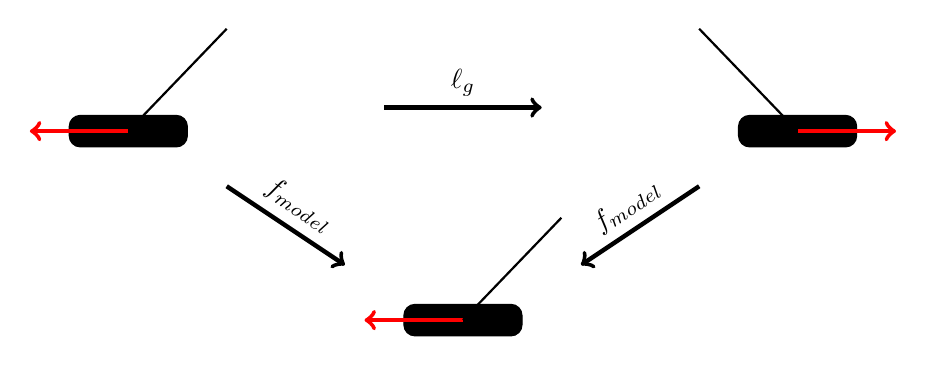
\begin{tikzpicture}
		\filldraw[black, rounded corners] (-5, 0) rectangle (-3.5, 0.4);
		\draw[black, thick] (-5 + 0.75, 0.2) -- (-3, 1.5);
		\draw[<-, red, ultra thick] (-5.5 , 0.2) -- ( -5 + 0.75, 0.2);
		%%%
		\filldraw[black, rounded corners] (5, 0) rectangle (5 - 1.5, 0.4);
		\draw[black, thick] (5 - 0.75, 0.2) -- (5 - 2, 1.5);
		\draw[<-, red, ultra thick] (5.5 , 0.2) -- ( 5 - 0.75, 0.2);
		%%%
		\draw[->, ultra thick] (-3, -.5) -- (-1.5, -1.5) node [sloped, midway, above] {$f_{model}$};
		\draw[->, ultra thick] (3, -.5) -- (1.5, -1.5) node [sloped, midway, above] {$f_{model}$};
		%%%
		\draw[->, ultra thick] (-1, 0.5) -- (1, 0.5) node [midway, above] {$\ell_g$};
		%%%
		\filldraw[black, rounded corners] (-.75, -2.4) rectangle (.75, -2);
		\draw[->, red, ultra thick] (-0 , -2.2) -- ( -1.25, -2.2);
		\draw[black, thick] (0, -2.2) -- (1.25,  -.9);

	\end{tikzpicture}
	\caption{Diagram of the MDP Homomorphism created by a world model, that is invariant to $\ell_g$,  the group actions .}
	\label{fig:invariant_world_model}
\end{figure}
\subsection{Approximate MDP Homomorphisms}
While they forgoe learning explcit symmetries \cite{van2020plannable}, they learn an Approximate MDP homomorphism. This approximation is exact in the case when the model fits the data perfectly.

In contrast to learning symmetires, they are looking to find a state and action embedding that is equivariant to the model, such that,
\begin{equation}
	Z(T(s, a)) = \overline{T}(Z(s), Z_s(a))
\end{equation}
Where $Z$ is the state embedding function, and $Z_s(a)$, is the action embedding function. Thus they construct and abstract MDP $\omc{M}$, with state space $\mathcal{Z}$ and action space $\omc{A}$, which they can act in. Further rather than using deep RL they discretise the state action space of the abstract MDP, $Z \rightarrow \mathcal{X}$, and use Value Iteration, repeated application of the bellman optimality operator, to learn the values of all state action pairs. From here, the value function can be interpolated to any abstract state action pair. Pseudocode for this process is given below. The world model for the MDP consists of four jointly trained networks, $Z$, $Z_a$, $\overline{T}$, $R_z(z)$, which are trained to minimise a bisimulation metric. A bisimulation metric measures how different the dynamics of two MDPs are.The bisimulation metric used is a squared distance between the abstract MDP and the origional MDP;
\begin{equation}
	L(\theta, \phi, \xi, \psi) = \sum_{(s', s, a) \sim \tau} d(Z_\theta (s'), \overline{T}_\phi(Z_\theta(s), Z_{a_\xi}(a))) +  d(R(s'), R_{z_\psi}(Z_\theta (s))) + C(\tilde{S})
\end{equation}
Where $d(z, z') = 1/2 (z - z')^2$ is the squared distance between two quantities. Additionally they add a contrastive term $C(\tilde{S})$, to stop trivial embeddings. $\tilde{S}$, is a set of randomly sampled states from the trajectory. The contrastive term, with model parameter dependence supressed, is given by,

\begin{equation}
	C(\tilde{S}) = \sum_{\tilde{s} \in \tilde{S}} \tilde{d}(Z_\theta(\tilde{s}), \overline{T}_\phi(Z(s), Z_{a_\xi}(a)))
\end{equation}
Here, $\tilde{d}(z, z') = max(0, \epsilon - d(z, z'))$, is a distance metric that encourages the embedding to not collapse to a point.
\begin{algorithm}
	\caption{Approximate MDP Homomorphism Pseudocode}
	\begin{algorithmic}
		\State Learn $Z: \mathcal{S} \rightarrow \mathcal{Z}$, $Z_a: \mathcal{A} \rightarrow \omc{A}$
		\State Discretise $\mathcal{Z}$ to $\mathcal{X}$.
		\State $Q(x, a) \leftarrow $ Plan in $\mathcal{X}$.
		\State $Q(z, a) \leftarrow$ Interpolate $Q(x, a)$
		\State $Q(s, a) = Q(Z(s), Z_a(a))$
	\end{algorithmic}
\end{algorithm}
This procedure produces impressive results, especially when limited to very few episodes of interaction with the MDP. Compared with a REINFORCE baseline, on 100 interactions of cartpole the episodice return is eight times higher. Additionally across a variety of tasks \cite{van2020plannable}, find a more structured latent space that with comparable world model methods, that use Encoder networks. There are however some limitations with the methods inability to generalise to stochastic transition dynmaics.


\section{Meta-Learning}
Meta Learning, is the process of learning to learn, across multiple tasks. This is a very broad field, where the goals are varied. Specifically, in this project, we are looking at parameter meta learning, where there is a single model, $f_\theta$, which is aplied to multiple different tasks, $\tau_i \sim \mathcal{T}$, drawn from a distriubtion.
On each task, there is a per task loss, $L_{\tau_i}(\theta)$, which is a function of the parameters of the model, and may change it's functional form.


The Model-Agnostic Meta-Learning(MAML) algorithm~\ref{alg:maml}, is the cannonical example of these methods. It works by performing a gradient based update on each task, storing the parameters,$\theta_i'$, of the model after each task's update, and then performs a gradient update on the meta loss, which is usually the sum of the per task losses $L_{\tau_i}(\theta_i')$, evaluated with their new parameters $\theta_i'$. This is then repeated till convergence. Pseudocode is given below.


\begin{algorithm}
	\caption{MAML Algorithm}
	\label{alg:maml}
	\begin{algorithmic}
		\State $\theta$ is randomly initialised
		\While{not done}
		\State Sample batch of tasks, $\tau_i \sim p(\tau)$
		\For {each task $\tau_i$}
		\State $\theta_i' \leftarrow \theta - \alpha \nabla_\theta L_{\tau_i}(F\theta)$
		\EndFor
		\State $\theta \leftarrow \theta - \beta \nabla_\theta \sum_{\tau_i \sim p(\tau)}{L_{\tau_i}(\theta_i')}$
		\EndWhile
	\end{algorithmic}
\end{algorithm}


\subsection{Meta-Learning Symmetries By Reparametrisation}
~\cite{zhou2020meta}, proposes a method to learn approximately equivarant networks, using the Model Agnostic Meta-Leaning~(MAML) framework~\cite{finn2017model}. MAML provides gradient updates to one set of parameters. However,~\cite{zhou2020meta} proposes a method of learning group convolutional layers~\ref{sec:G-CNNs}. This is achieved by breaking the model into two sets of parameters, the convolutional filters which are the conventionally trainable weights, and then the parameter sharing scheme. This is the non trainable part of a general $G-CNN$.

By reparameterising $\mat{W} \in \mathbb{R}^{m \times n}$ of a feedforward network, into a filter $v$ and a parameter sharing scheme $\mat{U}$;
\begin{equation}
	\text{vec}(\mat{W}) = \mat{U}v
\end{equation}
One can see this in the case of a group specific $\mat{U}_g$, is a way of representing a group convolutional layer.
An example of the eqivalence of this to the G-CNN scheme is for $C_2$, where the network is equivariant to an inversion of the input,
\begin{align}
	\mat{U_{C_2}}   & \cdot v  = [\oplus_{g \in C_2} \pi_g] \cdot v, \\
	\begin{pmatrix}
		1  & 0  \\
		0  & 1  \\
		-1 & 0  \\
		0  & -1 \\
	\end{pmatrix} & \cdot
	\begin{pmatrix}
		v_1 \\
		v_2 \\
	\end{pmatrix}
	= \begin{pmatrix}
		  v_1  \\
		  v_2  \\
		  -v_1 \\
		  -v_2 \\
	  \end{pmatrix}.
\end{align}
To prove this is equivariant, we can show that the following holds,
\begin{equation}
	\begin{pmatrix}
		0 & 1 \\
		1 & 0 \\
	\end{pmatrix} \cdot \left[
		\begin{pmatrix}
			v_1  & v_2  \\
			-v_1 & -v_2 \\
		\end{pmatrix} \cdot x \right] = \begin{pmatrix}
		-v_1 x_1 - v_2 x_2 \\
		v_1 x_1 + v_2 x_2  \\
	\end{pmatrix}
	= \begin{pmatrix}
		v_1  & v_2  \\
		-v_1 & -v_2 \\
	\end{pmatrix} \cdot  -x
\end{equation}
From this insight, they propose a method of meta-learning an equivariant parameter sharing scheme $\mat{U}$, given a set of tasks $\mathcal{T}$, that all posess the same equivarances.
Using an adapted MAML framework, $v$ is trained on a per task loss $L_{\tau_i}$ and the training data and $\mat{U}$ is trained on the meta loss on the validation data, they demonstrate the ability to recover the equivariant parameter sharing scheme, for convolutional layers.


\section{Other Related Works}
In Recent Reinforcement Learning another approach that is related to learning an MDP homomorphism from a world model \cite{mavor2022simple}, learns transitions between states, that have the same value, and as such they learn an approximate MDP Homomorphism. This is achieved by learning the reverse transition from a given state, in much the same way as $T(s', s, a)$ is learned from experience in a replay buffer.  

Another related recent development is that of \cite{rezaei2022continuous}, they prove that the MDP homomorphism results of Optimal Value equivalence are also found in the continuous action case. Further, they use this result in conjunction with DDPG\cite{lillicrap2015continuous} to learn a continuous action MDP Homomorphism, building a world model with a lax bisimulation metric, that is similar to the one used in \cite{van2020plannable}.

In wider machine learning using symmetry as an inductive bias is not new, and more generally requiring equivariance to input transofrmation is a key concept in modern Deep Learning. Recently the field of Geometricy Deep Learning has emerged as a unified formalism for deep learning on structured data, such as graphs, sets, Groups, and others.

Geometric Deep Learning is a field that provides a theoretical commonality for many successful network architectures, and has unified disperate architectures \cite{bronstein2021geometric}, such as Transformers and C-NNs, under a common framework. Geometric Deep learning provides a way to generalise the different inductive biases that arise from the wold. For example the translation invariance in object detection, or order permutation in Graphs.

A recent success in this field is the $\text{SE}(3)$-Transformer, \cite{fuchs2020se}, provides an equivaraint architecture, to $\text{SE}(3)$ transformations. This ensures that global rotations and translations on graphs or point clouds respond in the same manner. This happens to be an impoprtant equivariance to encode when dealing with proteins and other chemical molecules.As an example this architecture was used in the Alpha Fold protein structure prediciton networks~\cite{jumper2021highly}.

Nother Networks, which take inspiration from Nother's theorem demonstrate the ability to meta learn symbolic conservation laws, from real world data~\cite{alet2021noether}. An example of this is recovering the Hamiltonian of a spring, from real world data. This is particularly impressive as the spring itself does not conserve energy, due to friciton, and so the network must learn the approximate conservation law. This is achived by meta learning a conservation loss, across multiple tasks.



